\section{Background: HippoRAG 2 Retrieval as Stages A--E}\label{sec:background}

All values below are read from the released code (\texttt{src/hipporag}, version 2.0.0a5, tag \texttt{upstream-base},
commit \texttt{d5c8329}); Table~\ref{tab:defaults} lists the defaults that matter for retrieval.

\textbf{Index.} An OpenIE pass extracts $(s, r, o)$ triples from every passage. Normalised subjects and objects become
phrase nodes and every passage becomes a passage node. A passage is linked to each phrase in its triples by an edge of
weight~1. Each triple adds a fact edge between its subject and object whose weight is the number of passages asserting
it (one source count per passage), so re-asserting a fact in more passages strengthens its edge. Synonym edges connect
phrase pairs with embedding cosine $\ge 0.8$. The graph is undirected; the relation label is not stored on the edge.
A second \texttt{index()} call adds only new passages, facts and phrases, and computes synonym edges only for the new
phrases.

\textbf{Retrieval} runs five stages per query (Fig.~\ref{fig:pipeline}):
\begin{itemize}
\item[A] \emph{Fact candidates.} All facts are scored by the dot product between the query embedding and each fact's
embedding, min--max normalised; the top \texttt{linking\_top\_k}$\,=5$ become candidates.
\item[B] \emph{Recognition filter.} One LLM call with a few-shot DSPy prompt keeps the candidates it judges relevant
(at most 5). If none survive, the query falls back to dense passage retrieval and stages C--D are skipped.
\item[C] \emph{Seeds.} Each subject and object of a kept fact receives the fact's score divided by the number of
passages containing that phrase, averaged over its occurrences; only the top 5 phrases keep their weight. Every passage
receives its min--max normalised dense score times \texttt{passage\_node\_weight}$\,=0.05$. Together these form the
reset vector.
\item[D] \emph{Personalized PageRank} over the weighted undirected graph (python-igraph, PRPACK), damping $0.5$.
\item[E] \emph{Top 5.} Passages are ranked by PPR score; the reader sees the top \texttt{qa\_top\_k}$\,=5$.
\end{itemize}

\begin{table}[t]
\centering
\caption{HippoRAG 2 retrieval defaults (code, \texttt{utils/config\_utils.py}), unchanged in every run here.}
\label{tab:defaults}
\resizebox{\columnwidth}{!}{%
\begin{tabular}{lll}
\toprule
Parameter & Value & Role \\
\midrule
\texttt{linking\_top\_k} & 5 & facts to the filter; facts and phrases kept \\
\texttt{passage\_node\_weight} & 0.05 & weight of dense scores in the reset \\
\texttt{damping} & 0.5 & PPR damping \\
\texttt{retrieval\_top\_k} & 200 & passages returned \\
\texttt{qa\_top\_k} & 5 & passages given to the reader \\
\texttt{synonymy\_edge\_sim\_threshold} & 0.8 & synonym-edge cosine threshold \\
\texttt{synonymy\_edge\_topk} & 2047 & neighbours searched (at most 100 kept) \\
\texttt{is\_directed\_graph} & false & undirected graph and PPR \\
\texttt{temperature} & 0 & OpenIE, filter and reader \\
\bottomrule
\end{tabular}}
\end{table}

\begin{figure*}[t]
\centering
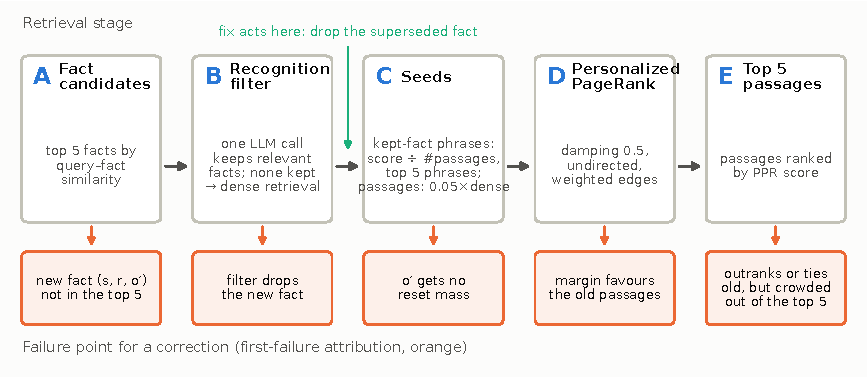
\includegraphics[width=0.9\textwidth]{figs/pipeline.pdf}
\caption{HippoRAG 2 retrieval as stages A--E (top) and the point at which a correction can be lost at each stage
(bottom), which defines the first-failure attribution of Section~\ref{sec:method}. The contradiction-aware fix acts
between B and C.}
\label{fig:pipeline}
\end{figure*}
